\subsection{Introduction}
The Lovász number $\vartheta$ is a well-known statistic of an arbitrary simple undirected graph $G$. 
As Lovász first observed in \cite{lovasz1979shannon}, one can define a number $\ltn(G)$ 
as the value of a certain semidefinite program (SDP) 
whose constraints depend on the adjacency matrix of $G$.
The Lovász number provides an upper bound on the Shannon capacity of the graph and satisfies the following inequalities:
\begin{equation}
\label{eq:theta_ineq}
\omega(G) \leq \ltn(\overline{G}) \leq \chi(G),
\end{equation}
where $\omega(G)$ is the size of the largest clique in $G$, $\chi(G)$ is the chromatic number of $G$, and $\overline{G}$ is the complement of $G$. 
This observation is remarkable, since $\vartheta$ is computable in polynomial time, while $\omega$ and $\chi$ are famously NP-hard to compute. 

The Lovász number has been studied for a variety of random graph models including the classical Erd\H{o}s-R\'{e}nyi (ER) random graph $G(n, p)$. 
Its expected value was first studied by Juh{\'a}sz~\cite{juhasz1982asymptotic}, 
who showed that $\E \ltn(G) = \Theta(\sqrt{n/p})$ for $\frac{\log^6 n}{n} \le p \le 1/2$. 
For $p=1/2$, Arora and Bhaskara~\cite{aroranote} showed that \(\ltn(G)\) concentrates around its median in an interval of polylogarithmic length.
In the sparse regime $p < n^{-1/2}$, it has been further shown that \(\ltn(G)\) concentrates around its median in an interval of constant length~\cite{coja2005lovasz}.
To the best of our knowledge, determining the correct constant in the $\Theta(\sqrt{n/p})$ asymptotic remains an open question. 

\begin{figure}[ht]
\centering
\begin{tabular}{cc}
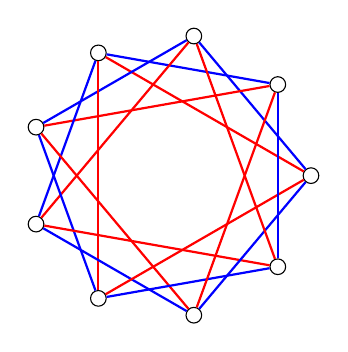
\begin{tikzpicture}[scale=1.2]
  \foreach \i in {0,...,8} {
    \node[draw, circle, inner sep=2pt] (v\i) at ({360/9 * \i}:1.5cm) {};
  }
  \foreach \i in {0,...,8} {
    \pgfmathtruncatemacro{\nextTwo}{mod(\i+2,9)}
    \draw[blue, thick] (v\i) -- (v\nextTwo);
    \pgfmathtruncatemacro{\nextThree}{mod(\i+3,9)}
    \draw[red, thick] (v\i) -- (v\nextThree);
  }
\end{tikzpicture}
&

\begin{tikzpicture}[every node/.style={minimum size=0.3cm, anchor=center, font=\footnotesize}, scale=0.6]
\matrix (m3) [matrix of nodes,
    left delimiter={(},
    right delimiter={)},
    row sep=-\pgflinewidth, column sep=-\pgflinewidth
]{
  $\cdot$ & $\cdot$ & $\textcolor{blue}{\mathbf{1}}$ & $\textcolor{red}{\mathbf{1}}$ & $\cdot$ & $\cdot$ & $\textcolor{red}{\mathbf{1}}$ & $\textcolor{blue}{\mathbf{1}}$ & $\cdot$ \\
  $\cdot$ & $\cdot$ & $\cdot$ & $\textcolor{blue}{\mathbf{1}}$ & $\textcolor{red}{\mathbf{1}}$ & $\cdot$ & $\cdot$ & $\textcolor{red}{\mathbf{1}}$ & $\textcolor{blue}{\mathbf{1}}$ \\
  $\textcolor{blue}{\mathbf{1}}$ & $\cdot$ & $\cdot$ & $\cdot$ & $\textcolor{blue}{\mathbf{1}}$ & $\textcolor{red}{\mathbf{1}}$ & $\cdot$ & $\cdot$ & $\textcolor{red}{\mathbf{1}}$ \\
  $\textcolor{red}{\mathbf{1}}$ & $\textcolor{blue}{\mathbf{1}}$ & $\cdot$ & $\cdot$ & $\cdot$ & $\textcolor{blue}{\mathbf{1}}$ & $\textcolor{red}{\mathbf{1}}$ & $\cdot$ & $\cdot$ \\
  $\cdot$ & $\textcolor{red}{\mathbf{1}}$ & $\textcolor{blue}{\mathbf{1}}$ & $\cdot$ & $\cdot$ & $\cdot$ & $\textcolor{blue}{\mathbf{1}}$ & $\textcolor{red}{\mathbf{1}}$ & $\cdot$ \\
  $\cdot$ & $\cdot$ & $\textcolor{red}{\mathbf{1}}$ & $\textcolor{blue}{\mathbf{1}}$ & $\cdot$ & $\cdot$ & $\cdot$ & $\textcolor{blue}{\mathbf{1}}$ & $\textcolor{red}{\mathbf{1}}$ \\
  $\textcolor{red}{\mathbf{1}}$ & $\cdot$ & $\cdot$ & $\textcolor{red}{\mathbf{1}}$ & $\textcolor{blue}{\mathbf{1}}$ & $\cdot$ & $\cdot$ & $\cdot$ & $\textcolor{blue}{\mathbf{1}}$ \\
  $\textcolor{blue}{\mathbf{1}}$ & $\textcolor{red}{\mathbf{1}}$ & $\cdot$ & $\cdot$ & $\textcolor{red}{\mathbf{1}}$ & $\textcolor{blue}{\mathbf{1}}$ & $\cdot$ & $\cdot$ & $\cdot$ \\
  $\cdot$ & $\textcolor{blue}{\mathbf{1}}$ & $\textcolor{red}{\mathbf{1}}$ & $\cdot$ & $\cdot$ & $\textcolor{red}{\mathbf{1}}$ & $\textcolor{blue}{\mathbf{1}}$ & $\cdot$ & $\cdot$ \\
};
\end{tikzpicture}
\\[0.0em]
\end{tabular}
\caption{Circulant graph on \(9\) vertices and its adjacency matrix (0's replaced by dots). Each vertex \(i\)  is connected to vertices \(\textcolor{blue}{i + 2, i+7}, \textcolor{red}{i + 3}\), and \(\textcolor{red}{i + 6} \mod 9\).}
\label{fig:circ_graphs}
\end{figure}
In this work, we focus on a class of random \emph{circulant} graphs (RCGs), a family of vertex-transitive graphs with a circulant adjacency matrix; see~\Cref{fig:circ_graphs} and~\Cref{def:circ_graph,def:rand_circ}. 
We emphasize that RCGs are fully determined by the connectivity of any given single vertex. Therefore, a dense RCG can be generated with \(\frac{n - 1}{2}\) random bits, where each bit affects the presence of \(n\) edges, in contrast to the \(\frac{n(n - 1)}{2}\) random bits in $G(n,1/2)$, each affecting just one edge.
In this sense, RCGs may be viewed as a ``partial derandomization'' of ER graphs.
Indeed, circulant graphs are precisely Cayley graphs on the group \(\mathbb{Z}_n\), and general random Cayley graphs have long been studied for similar purposes in theoretical computer science.


It is therefore of interest to understand to what extent the above results for ER graphs also apply to RCGs.
For dense RCGs, the asymptotics of the clique number and the chromatic number are well-understood:~\cite{green2005counting} showed a high-probability upper bound on the clique number \(\omega(G) = O(\log n)\), and later~\cite{green2016counting} proved that the chromatic number is at most $(1+o(1)) \frac{n} { 2 \log_2 n}$ with high probability. 
These results imply bounds on the Lovász number through~\Cref{eq:theta_ineq}, but the resulting upper and lower bounds are far apart.

Our main result is much sharper upper and lower bounds on the expected Lovász number of a dense RCG. 
\begin{theorem}
\label{thm:main}
    There exists a constant $C > 0$ such that, for a dense random circulant graph \(G\) on $n$ vertices (\Cref{def:rand_circ}),
    \begin{equation}
        \sqrt{n} \leq \E \ltn(G) \leq C \sqrt{n \log \log n}.
    \end{equation}
\end{theorem}

\noindent
\emph{Proof Strategy:}
Our proof of the upper bound in~\Cref{thm:main} relies on the algebraic structure of circulant graphs. First, following~\cite{magsino2019linear}, we transform the SDP formulation of \(\ltn(G)\) to a linear program (LP) using the fact that the circulant matrices are diagonalizable by a discrete Fourier transform (DFT)
\Cref{lem:lp_with_g} gives the resulting LP:
\begin{equation}
\label{eq:first_step}
\begin{aligned}
    \ltn(G) &= \max_{(y_0, \dots, y_{n-1}) \in \R^{n}} \braket{y, g}, \\ \text{ subject to }
    &\begin{cases} y_k = y_{n - k} \text{ for } k = 1,\ldots, n - 1, \\
    \norm{y}_1 = 1,
    y \geq \mathbf{0}, \\
    \braket{y, f_k} = 0\text{ for all edges } (0, k).
    \end{cases}
\end{aligned}
\end{equation}
Here, \(f_k\) is the \(k\)-th row of the DFT matrix \(F\), and \(g \coloneqq Fb\) for \(b \in \{\pm 1\}^{n}\) with $b_0=1$ and \(b_k = 1\) if \((0, k)\) is not an edge, and \(-1\) otherwise, for $1 \le k \le n-1$. We denote \(\mathbf{0} \coloneqq (0, \ldots, 0)\) and \(y \geq \mathbf{0}\) stands for entrywise positivity of \(y\).

The last constraint in~\Cref{eq:first_step} requires the Fourier transform of \(y\) to have a specific sparsity pattern. Uncertainty principles for the Fourier transform (see, e.g.,~\cite{bandeira2018discrete}) then suggest that all feasible vectors \(y\) must be dense \cite{demanet2014scaling}.
A quantitative version of this ``density'' would be enough to bound the LP.
To illustrate, suppose that $y$ is a feasible vector with $\|y\|_1 = 1$ and its mass is spread almost uniformly among its coordinates, i.e., that
\(\norm{y}_2 \leq \frac{c}{\sqrt{n}} \norm{y}_1 = \frac{c}{\sqrt{n}}\), for some constant \(c > 0\). Since \(\norm{g}_2 = n\), Cauchy-Schwarz inequality would give \(\braket{y, g} \leq \norm{y}_2 \norm{g}_2 \leq c\sqrt{n},\) proving upper bound in~\Cref{thm:main} without the extra \(\sqrt{\log \log n}\) factor.

The second part of our proof,~\Cref{lem:rip}, makes the aforementioned intuition rigorous, relying on the \textit{restricted isometry property} (RIP,~\Cref{def:rip}).
The $f_k$ in our constraints form a so-called \emph{subsampled DFT basis}, which is a random subset of the Fourier basis.
The RIP for such bases is in fact a celebrated topic in the compressed sensing literature. RIP was first introduced and studied for subsampled DFT bases in seminal work of Candès and Tao~\cite{candes2006near},
and since then, one of the central 
questions for compressed sensing is 
the number of $f_k$ needed for RIP to hold. 
\Cref{lem:rip_dft} describes a simplified version of the current best bound due to~\cite{haviv2017restricted} which is sufficient for our purposes.
Interestingly, our upper bound proof only uses the fact that feasible solutions of~\Cref{eq:first_step} lie on a (random) nullspace of a subsampled DFT matrix, and omits the positivity constraint \(y \geq \mathbf{0}\). However, as we discuss in~\Cref{sec:discussion}, we believe that this constraint is important for tighter results.
